\subsection{Farbigkeit}
\authors{Ole Simmering, Lena Prahe}

Im siebten Teilexperiment wurden die Photographien des sechsten Versuches genutzt und auf die Farbe der Reaktion untersucht. Im Folgenden sind die RGB-Werte, also die Rot-, Grün- und Blauanteile und die entsprechenden HSL-Werte, also der Farbwert, der Sättigungswert und der Helligkeitswert dargestellt (siehe Tab. \ref{RGB-Werte_Tabelle} und Abb. \ref{Diagramm_H_ueber_t}). Der Farbwert wird als Farbwinkel H auf dem Farbkreis (etwa 0$^\circ$ für Rot, 120$^\circ$ für Grün, 240$^\circ$ für Blau) angegeben. So konnten wir mit dem Farbwert der Reaktion vergleichen, wie sich die Farbe über die Zeit verändert, ohne den Intensitätsverlauf zu berücksichtigen.

\begin{dsatable}
 \centering
 \caption{RGB-Werte und HSL-Werte der Bilder von der Reaktion.}
 \begin{tabular}{lcc} % vier Spalten
  \toprule
   Zeit  & RGB & HSL\\
  \midrule
   nach 2 s  & 2, 125, 124 &   180, 96.9\%, 24.9\%    \\
   nach 4 s  & 2, 83, 86   &   182, 95.5\%, 17.3\%    \\
   nach 6 s  & 1, 48, 58   &   191, 96.6\%, 11.6\%    \\
   nach 8 s  & 1, 31, 42   &   196, 95.3\%, 8.4\%     \\ 
  \bottomrule
 \end{tabular}
 \label{RGB-Werte_Tabelle}
 
\end{dsatable}

\begin{dsafigure}
	\centering
	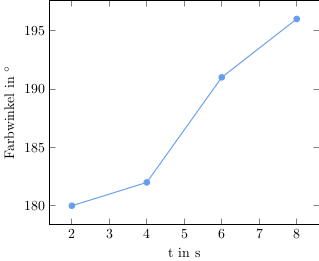
\includegraphics[width=7cm]{figure0.png}
	\label{Diagramm_H_ueber_t}
	\caption{Abhängigkeit des Farbwinkels im Farbkreis von der Zeit.}
\end{dsafigure}

Diese Werte ergaben sich aus einer Analyse der RGB-Werte eines fixen Bildpunktes in der Bilderserie der Reaktion mithilfe des Grafikeditors GIMP \cite{GIMP}. Die RGB-Werte wurden mittels des Online-Rechners RapidTables \cite{RapidTables} zu HSL umgerechnet. Es ist erkennbar, dass sich der Farbwinkel fast nicht ändert (siehe Abb. \ref{Diagramm_H_ueber_t}). Es ist vermutlich nur ein Stoff für die Farbgebung verantwortlich, da die Farbe des Lichtes fast konstant bleibt.
